\chapter{Kinetische energie en verkeersveiligheid}\label{ch:g9:kinetic-energy-safety}

Sinds het opwindspeelgoed uit je kindertijd is \omterm{def:g5:everyday-energy:energy}{energie} een verhaal
van voorraden en vormen geweest --- levendig, nuttig en zonder
getallen. Dat wachten houdt nu op. De \omterm{def:g5:everyday-energy:energy}{energie} van beweging
krijgt haar formule, \omterm{def:g5:everyday-energy:energy}{energie} krijgt haar
\omterm{def:g6:measurement-in-science:measuring}{eenheid}, en de rekenkunde blijkt een zaak van leven en dood te
regeren: waarom een auto op dubbele \omterm{def:g7:motion-average-speed:formula}{snelheid} vier keer zo
moeilijk te stoppen is, en wat één \omterm{def:g2:measuring-time:second}{seconde} onoplettendheid kost in
\omterm{def:g2:measuring-length:units}{meters}.

\section{De energie van beweging}

\begin{definition}[De joule]\label{def:g9:kinetic-energy-safety:joule}
\omterm{def:g5:everyday-energy:energy}{Energie} --- in elke vorm --- wordt gemeten in
\emph{joule}\index{joule} (\unit{J}), ter ere van de experimentator die
bewees dat \omterm{def:g5:heat-and-insulation:heat}{warmte} zelf een vorm van \omterm{def:g5:everyday-energy:energy}{energie} is.
Ankers: dit boek van de vloer op de plank tillen kost een paar joule;
een kloppend hart ongeveer één joule per slag; een reep chocolade slaat
een miljoen joule voedselenergie op.
\end{definition}

\begin{proposition}[Kinetische energie]\label{prop:g9:kinetic-energy-safety:formula}
Een lichaam met \omterm{def:g3:measuring-mass:mass}{massa} $m$ (in \unit{kg}) dat met
\omterm{def:g7:motion-average-speed:formula}{snelheid} $v$ (in \unit{m/s}) beweegt, draagt op grond van zijn
beweging de \emph{kinetische energie}\index{kinetische energie}
\[
E_k = \frac{1}{2} \times m \times v^2 ,
\]
in \omterm{def:g9:kinetic-energy-safety:joule}{joule}. Twee knoppen, ongelijke machten: de
\omterm{def:g3:measuring-mass:mass}{massa} verdubbelen verdubbelt $E_k$ --- maar de
\emph{\omterm{def:g7:motion-average-speed:formula}{snelheid}} verdubbelen \emph{verviervoudigt} haar, want de
\omterm{def:g7:motion-average-speed:formula}{snelheid} staat er gekwadrateerd in.
\omterm{def:g7:motion-average-speed:formula}{Snelheid} is de gevaarlijke knop.
\end{proposition}

\begin{example}[Eerste berekeningen]\label{ex:g9:kinetic-energy-safety:first}
Een voetbal van \qty{0.45}{kg} op \qty{20}{m/s}: $E_k = 0.5 \times
0.45 \times 20^2 = \qty{90}{J}$. Een sprinter van \qty{60}{kg} op
\qty{10}{m/s}: $0.5 \times 60 \times 100 = \qty{3000}{J}$. Een auto van
\qty{1000}{kg} op \qty{50}{km/h} --- eerst omrekenen: $50 \div 3.6
\approx \qty{13.9}{m/s}$ --- $E_k = 0.5 \times 1000 \times 13.9^2
\approx \qty{9.7e4}{J}$: bijna honderdduizend \omterm{def:g9:kinetic-energy-safety:joule}{joule}. Dezelfde
auto op \qty{100}{km/h}: vier keer zoveel --- \qty{3.9e5}{J}. De
waarschuwing van de formule, in getallen.
\end{example}

\begin{omfigure}
\begin{tikzpicture}
\begin{axis}[omaxis, width=10.2cm, height=6.0cm,
    xlabel={snelheid $v$ (\unit{km/h})},
    ylabel={$E_k$ (\unit{kJ})},
    xtick={0,30,50,70,90,110,130}, ytick={0,100,200,300,400,500},
    ymin=0, ymax=560, xmin=0, xmax=140, samples=100]
  \addplot[very thick, omThm, domain=0:135]
    {0.5*1000*(x/3.6)^2/1000};
  \addplot[only marks, mark=*, omDef] coordinates
    {(50,96.5) (100,385.8)};
  \node[right, font=\small, omDef] at (axis cs:38,130)
    {\qty{50}{km/h}};
  \node[left, font=\small, omDef] at (axis cs:99,400)
    {\qty{100}{km/h}: viervoudig};
\end{axis}
\end{tikzpicture}

{\small De \omterm{prop:g9:kinetic-energy-safety:formula}{kinetische energie} van een auto van één ton tegen de
\omterm{def:g7:motion-average-speed:formula}{snelheid}: geen lijn maar een parabool --- het kwadraat uit de
formule, getekend. Verdubbel de \omterm{def:g7:motion-average-speed:formula}{snelheid} en je moet vier keer
zoveel \omterm{def:g5:everyday-energy:energy}{energie} kwijtraken.}
\end{omfigure}

\begin{example}[Waar het remmen haar naartoe stuurt]\label{ex:g9:kinetic-energy-safety:brakes}
Om te stoppen moet een auto zijn hele $E_k$ aan iets overdragen ---
\omterm{def:g5:everyday-energy:energy}{energie} wordt doorgegeven, nooit uitgewist, zoals de ketens uit
je kindertijd volhielden. De greep van de remmen zet haar om in
\omterm{def:g5:heat-and-insulation:heat}{warmte}: schijven gloeien amberkleurig na afdalingen in de
bergen, en de geur van hete remmen \emph{is} \omterm{prop:g9:kinetic-energy-safety:formula}{kinetische energie}
die met pensioen gaat. Bij een botsing is de overdracht gewelddadig en
ogenblikkelijk --- in gekreukeld staal. Elk verkeersveiligheidsgetal
hieronder is deze boekhouding: hoe groter de $E_k$, hoe langer, of hoe
lelijker, haar pensionering.
\end{example}

\begin{omfigure}
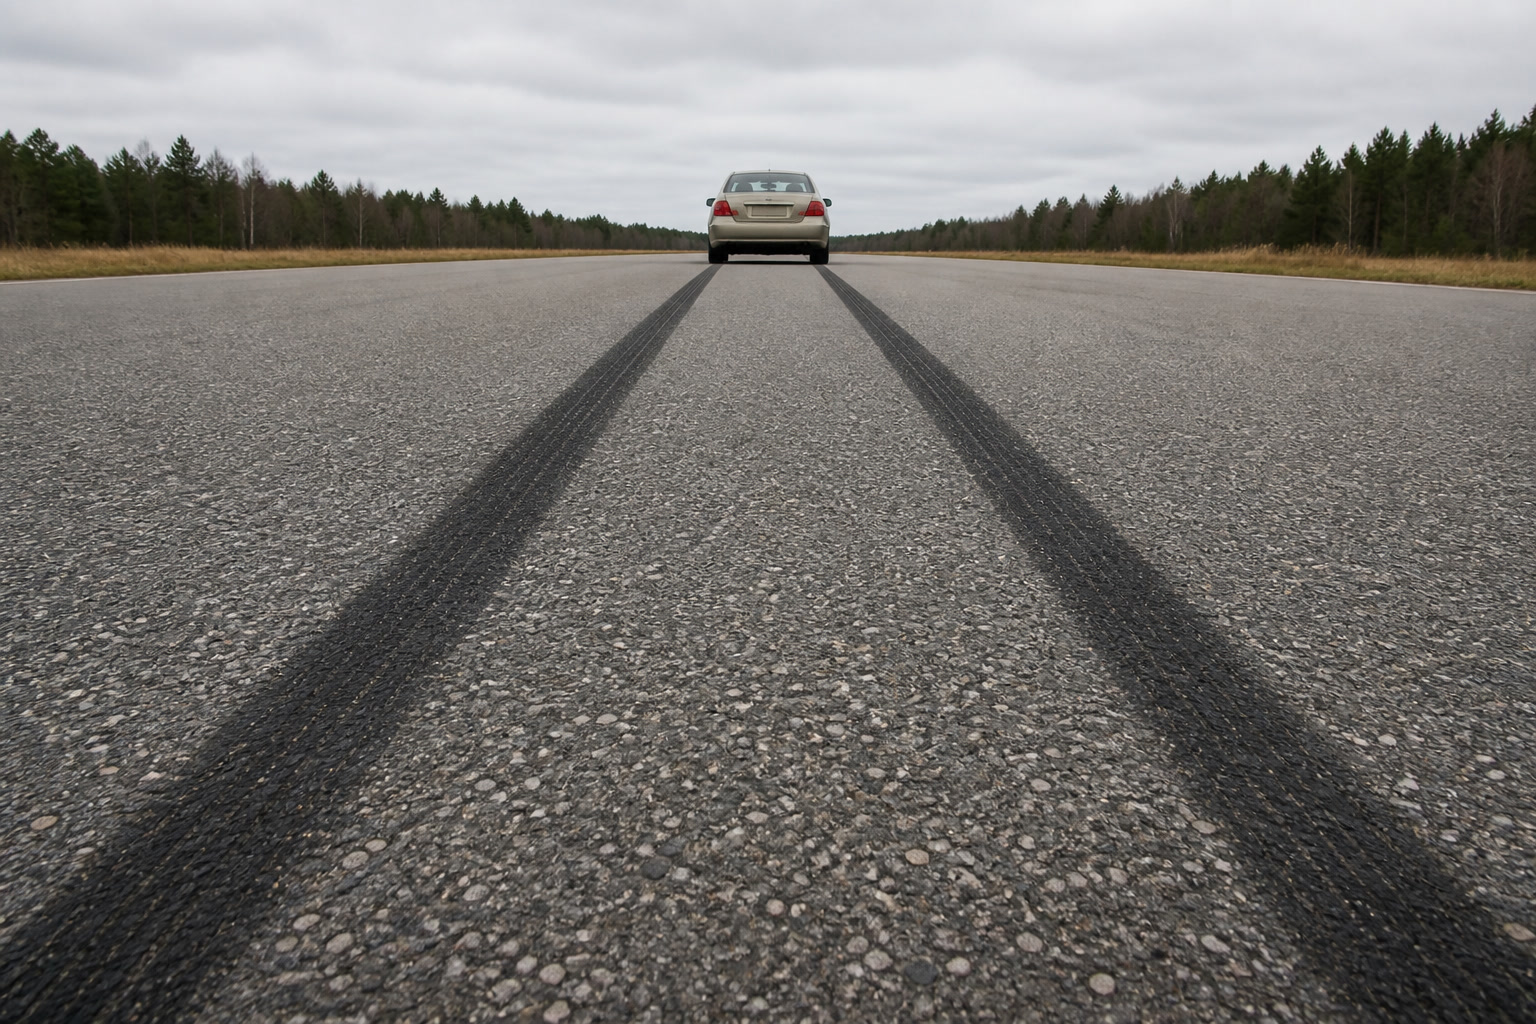
\includegraphics[width=0.55\linewidth]{images/book1/ai/g9-kinetic-skid-marks.jpg}

{\small Waar de \omterm{prop:g9:kinetic-energy-safety:formula}{kinetische energie} bleef: de remmen en de weg maakten er \omterm{def:g5:heat-and-insulation:heat}{warmte} van, en de banden tekenden het ontvangstbewijs.}
\end{omfigure}

\section{De stopafstand}

\begin{proposition}[Stoppen = denken + remmen]\label{prop:g9:kinetic-energy-safety:stopping}
Een bestuurder die gevaar opmerkt, stopt pas na twee stukken weg:
\begin{enumerate}
  \item de \emph{reactieafstand}\index{reactieafstand}: de weg die
        wordt afgelegd terwijl het brein het opmerkt en de voet
        beweegt --- ongeveer één volle \omterm{def:g2:measuring-time:second}{seconde} op onveranderde
        \omterm{def:g7:motion-average-speed:formula}{snelheid}, dus dit stuk groeit \emph{evenredig} met
        $v$;
  \item de \emph{remweg}\index{remweg}: de weg die de remmen nodig
        hebben om de \omterm{prop:g9:kinetic-energy-safety:formula}{kinetische energie} met pensioen te sturen ---
        en omdat $E_k$ de $v^2$ meedraagt, groeit dit stuk met het
        \emph{kwadraat} van de \omterm{def:g7:motion-average-speed:formula}{snelheid}: dubbele
        \omterm{def:g7:motion-average-speed:formula}{snelheid}, viervoudige \omterm{prop:g9:kinetic-energy-safety:stopping}{remweg}.
\end{enumerate}
Hun som, de \emph{stopafstand}, is het getal dat het kind ontmoet dat
achter de bal aan rent.
\end{proposition}

\begin{example}[De tabel die elke bestuurder zou moeten bezitten]\label{ex:g9:kinetic-energy-safety:table}
Droge weg, oplettende bestuurder (reactie van één \omterm{def:g2:measuring-time:second}{seconde}; goede
remmen):
\begin{center}
\begin{tabular}{l|c|c|c}
\omterm{def:g7:motion-average-speed:formula}{snelheid} & reactie & remmen & stoppen \\
\hline
\qty{50}{km/h} & \qty{14}{m} & \qty{13}{m} & \qty{27}{m} \\
\qty{90}{km/h} & \qty{25}{m} & \qty{40}{m} & \qty{65}{m} \\
\qty{130}{km/h} & \qty{36}{m} & \qty{85}{m} & \qty{121}{m}
\end{tabular}
\end{center}
Lees hem twee keer. Bij stadssnelheid anderhalve buslengte; bij
snelwegsnelheid een volledige atletiekbaan plus een vijfde. En
de verhoudingen bevestigen de twee wetten: de reactie groeit als $v$,
het remmen als $v^2$ --- bij hoge \omterm{def:g7:motion-average-speed:formula}{snelheid} verslindt het remmen
het totaal.
\end{example}

\begin{method}[Een stopafstand schatten]\label{met:g9:kinetic-energy-safety:estimate}
\begin{enumerate}
  \item reken de \omterm{def:g7:motion-average-speed:formula}{snelheid} om naar \unit{m/s} (deel \unit{km/h}
        door $3.6$);
  \item \omterm{prop:g9:kinetic-energy-safety:stopping}{reactieafstand}: de weg van één \omterm{def:g2:measuring-time:second}{seconde} --- het getal in
        \unit{m/s} zelf, in \omterm{def:g2:measuring-length:units}{meter};
  \item \omterm{prop:g9:kinetic-energy-safety:stopping}{remweg}: schaal een bekend anker met het kwadraat ---
        vanaf \qty{13}{m} bij \qty{50}{km/h}, vermenigvuldig met
        $(v/50)^2$;
  \item tel op, en vergelijk met wat de weg voor je werkelijk biedt.
\end{enumerate}
Natte wegen verdubbelen het aandeel van het remmen; vermoeide of
afgeleide bestuurders rekken de reactieseconde naar twee --- maak de som
opnieuw met de eerlijke invoer.
\end{method}

\begin{example}[De prijs van een blik]\label{ex:g9:kinetic-energy-safety:glance}
Een blik van twee \omterm{def:g2:measuring-time:second}{seconden} op een telefoon bij \qty{90}{km/h}: de auto
legt $2 \times 25 = \qty{50}{m}$ af --- een half voetbalveld --- blind
gereden, nog voor er ook maar een reactieseconde begint. Bij
stadssnelheid verspilt dezelfde blik blind \qty{28}{m}: voorbij
de kruising, voorbij het schoolhek. Het gevaarlijkste onderdeel van de
auto wordt door geen enkele formule hier gemeten: de aandacht van de
bestuurder.
\end{example}

\begin{remark}[Gordels, airbags en helmen]\label{rem:g9:kinetic-energy-safety:belts}
Bij een botsing stopt de auto in een \omterm{def:g2:measuring-length:units}{meter} kreukelen --- maar
een niet-gegordelde inzittende gaat op volle \omterm{def:g7:motion-average-speed:formula}{snelheid} door (de
stille zin van het vorige hoofdstuk, grimmig toegepast) tot hij wordt
gestopt door wat er komt: dashboard, voorruit, wegdek. Veiligheidsgordels
en airbags stoppen het lichaam over een langere afstand en tijd en
sturen zijn \omterm{prop:g9:kinetic-energy-safety:formula}{kinetische energie} zachtjes met pensioen in plaats
van in één klap; de helm van de fietser doet hetzelfde voor de
onvervangbare inhoud van de schedel, en zijn indrukbare schuim koopt
\omterm{def:g2:measuring-length:units}{centimeters} zacht stoppen. Geen van alle vermindert je $E_k$ met
één \omterm{def:g9:kinetic-energy-safety:joule}{joule} --- ze beschaven haar pensionering.
\end{remark}

\section{Oefeningen}

\begin{exercise}[$\star$]\label{exo:g9:kinetic-energy-safety:1}
Geef de \omterm{def:g6:measurement-in-science:measuring}{eenheid} van \omterm{def:g5:everyday-energy:energy}{energie} en twee ankers ervoor,
en schrijf de formule voor de \omterm{prop:g9:kinetic-energy-safety:formula}{kinetische energie} met haar
eenheden op.
\end{exercise}

\begin{exercise}[$\star$]\label{exo:g9:kinetic-energy-safety:2}
Bereken $E_k$: een haas van \qty{2}{kg} op \qty{10}{m/s}; een
rugbyspeler van \qty{80}{kg} op \qty{5}{m/s}.
\end{exercise}

\begin{exercise}[$\star$]\label{exo:g9:kinetic-energy-safety:3}
Wat verhoogt de $E_k$ van een auto meer: de helft van zijn
\omterm{def:g3:measuring-mass:mass}{massa} aan lading erbij, of zijn \omterm{def:g7:motion-average-speed:formula}{snelheid} met de helft
verhogen? Toon beide factoren.
\end{exercise}

\begin{exercise}[$\star$]\label{exo:g9:kinetic-energy-safety:4}
Noem de twee stukken van de stopafstand en hun groeiwetten --- de ene
evenredig, de andere kwadratisch.
\end{exercise}

\begin{exercise}[$\star$]\label{exo:g9:kinetic-energy-safety:5}
Uit de tabel van de bestuurder: welk deel van de stopafstand is remmen
bij \qty{50}{km/h} --- en bij \qty{130}{km/h}? Wat is er veranderd?
\end{exercise}

\begin{exercise}[$\star$]\label{exo:g9:kinetic-energy-safety:6}
Waar gaat de \omterm{prop:g9:kinetic-energy-safety:formula}{kinetische energie} van een remmende auto heen? Noem
de geur en de gloed --- en de wet uit je kindertijd die verbiedt dat ze
zomaar verdwijnt.
\end{exercise}

\begin{exercise}[$\star$]\label{exo:g9:kinetic-energy-safety:7}
Bereken de \omterm{prop:g9:kinetic-energy-safety:stopping}{reactieafstand} bij \qty{36}{km/h}, \qty{72}{km/h} en
\qty{108}{km/h} (één oplettende \omterm{def:g2:measuring-time:second}{seconde}). Volgens welk eenvoudig patroon
marcheren de antwoorden?
\end{exercise}

\begin{exercise}[$\star$]\label{exo:g9:kinetic-energy-safety:8}
Waarom vermindert een veiligheidsgordel je \omterm{prop:g9:kinetic-energy-safety:formula}{kinetische energie}
niet --- en wat beschaaft hij in plaats daarvan?
\end{exercise}

\begin{exercise}[$\star\star$]\label{exo:g9:kinetic-energy-safety:9}
De \omterm{prop:g9:kinetic-energy-safety:stopping}{remweg} van een scooter is \qty{8}{m} bij \qty{30}{km/h}.
Schat hem bij \qty{60}{km/h} en bij \qty{90}{km/h} --- en noem de wet
waarmee je schaalde.
\end{exercise}

\begin{exercise}[$\star\star$]\label{exo:g9:kinetic-energy-safety:10}
Gemeenteraden verlagen de limiet in schoolzones van \qty{50}{} naar
\qty{30}{km/h}. Vergelijk de twee stopafstanden (anker: \qty{13}{m}
remmen bij $50$; reactie van één \omterm{def:g2:measuring-time:second}{seconde}) --- en de twee kinetische
energieën. Welke vergelijking vind je overtuigender op een poster?
\end{exercise}

\begin{exercise}[$\star\star$]\label{exo:g9:kinetic-energy-safety:11}
Regen verdubbelt \omterm{prop:g9:kinetic-energy-safety:stopping}{remwegen}. Bouw de stopkolom van de tabel van
de bestuurder opnieuw op voor natte wegen bij $50$ en \qty{90}{km/h} ---
welk onderdeel heb je verdubbeld, welk niet, en waarom?
\end{exercise}

\begin{exercise}[$\star\star\star$]\label{exo:g9:kinetic-energy-safety:12}
Een vrachtwagen van \qty{20000}{kg} rolt met \qty{90}{km/h}. Bereken
zijn $E_k$ in wetenschappelijke notatie; vind de \omterm{def:g7:motion-average-speed:formula}{snelheid}
waarbij een auto van \qty{1000}{kg} die \omterm{def:g5:everyday-energy:energy}{energie} zou evenaren
(stel de twee formules gelijk --- de algebra is dit jaar aan jou); en
concludeer waarom er op bergwegen uitwijkstroken voor op hol geslagen
vrachtwagens bestaan terwijl geen enkele strook auto's bedient.
\end{exercise}

\section{Probleem: de veiligheidscampagne}

\begin{problem}[{Weekendprobleem --- de klas ontwerpt de
verkeersveiligheidscampagne van de stad; posters gecontroleerd met de
formule; de lastige vragen van de burgemeester}]\label{pb:g9:kinetic-energy-safety:1}
De stad geeft opdracht voor een campagne, op één voorwaarde: elk getal
op elke poster moet een natuurkundige controle doorstaan. De klas
rekent. (Ankers: reactie één \omterm{def:g2:measuring-time:second}{seconde}; remmen \qty{13}{m} bij
\qty{50}{km/h}, geschaald met het kwadraat; \omterm{def:g3:measuring-mass:mass}{massa} van de auto
\qty{1000}{kg}.)

\medskip\noindent\textbf{Deel I --- Poster één: ``50 en geen 60''.}
\begin{enumerate}
  \item Bereken beide snelheden in \unit{m/s} (één decimaal).
  \item \omterm{prop:g9:kinetic-energy-safety:stopping}{Reactieafstanden} bij beide snelheden?
  \item \omterm{prop:g9:kinetic-energy-safety:stopping}{Remwegen} bij beide (schaal het anker)?
  \item De kop van de poster: ``Tien eenheden
        \omterm{def:g7:motion-average-speed:formula}{snelheid} erbij --- hoeveel \omterm{def:g2:measuring-length:units}{meter} stoppen
        erbij?'' Vul het getal in.
\end{enumerate}

\medskip\noindent\textbf{Deel II --- Poster twee: ``De muur van
\omterm{def:g7:motion-average-speed:formula}{snelheid}''.}
Het ontwerp toont botsenergieën als valhoogtes: een botsing bij
\omterm{def:g7:motion-average-speed:formula}{snelheid} $v$ ``staat gelijk aan'' een val van de hoogte waarbij
dezelfde \omterm{def:g5:everyday-energy:energy}{energie} zou worden gewonnen.
\begin{enumerate}[resume]
  \item Bereken de $E_k$ van de auto bij \qty{50}{km/h} (uit Deel I)
        en bij \qty{90}{km/h}.
  \item De vormgevers hebben hoogtes nodig: een val van \qty{1}{m}
        levert deze auto ongeveer \qty{9.8}{kJ} op ($m g h$ --- de
        andere formule van het volgende hoofdstuk, vroeg geleend). Met
        welke valhoogtes komen de twee botsenergieën overeen? (Deel;
        rond af op de \omterm{def:g2:measuring-length:units}{meter}.)
  \item Welke alledaagse gebouwen passen bij die hoogtes? Stel de
        regel voor de poster op.
  \item De burgemeester werpt tegen: ``Niemand rijdt tegen muren;
        auto's kreukelen, gordels vangen op.'' Verdedig de natuurkunde
        van de poster terwijl je zijn punt toegeeft --- wat veranderen
        kreukelzones en gordels, en welk getal veranderen ze niet?
\end{enumerate}

\medskip\noindent\textbf{Deel III --- Poster drie: ``Eén \omterm{def:g2:measuring-time:second}{seconde}''.}
\begin{enumerate}[resume]
  \item Hoeveel \omterm{def:g2:measuring-length:units}{meter} kost bij \qty{90}{km/h} één afgeleide
        \omterm{def:g2:measuring-time:second}{seconde}, nog voor er wordt geremd? En een telefoonblik van twee
        \omterm{def:g2:measuring-time:second}{seconden}?
  \item De variant met de vermoeide bestuurder: de reactie gerekt tot
        twee \omterm{def:g2:measuring-time:second}{seconden}. Bereken de volledige stopafstand bij
        \qty{90}{km/h} opnieuw en vergelijk met de \qty{65}{m} van de
        oplettende bestuurder.
  \item Een sceptisch raadslid: ``Eén \omterm{def:g2:measuring-time:second}{seconde} zal naast die grote
        remgetallen toch weinig uitmaken.'' Bij welke
        snelheden heeft hij het het meest mis --- lage of hoge?
        (Vergelijk de groeiwetten van de twee onderdelen.)
  \item Teken af voor de campagne: drie slotregels onder aan de
        posters, één per poster, elk met haar formule in gewone
        woorden.
\end{enumerate}
\end{problem}
